\chapter{Sistemas imunológicos e a Teoria do Perigo}

O primeiro modelo do sistema imunológico foi o da distinção entre o próprio e o não-próprio, proposto por Burnet\footnote{BURNET, F. M. 1959. \emph{The Clonal Selection Theory of Acquired Immunity}.}. Ao longo do tempo, novos modelos foram criados, tentando resolver as questões que os outros modelos não explicavam, destancando-se o modelo do não-próprio infeccioso, de Janeway\footnote{JANEWAY, C. A. 1989. \emph{Approaching the Asymptote? Evolution and Revolution in Immunology}.}.

\section{Discriminação do próprio e não-próprio}

Nesse modelo, existia apenas um tipo de linfócito, o linfócito B, repsonsável por identificar os antígenos e produzir os respectivos anticorpos. A resposta imune adaptativa era gerada apenas pela identificação desses antígenos, sem qualquer mecanismo de controle.

\begin{figure}[h]
\centering
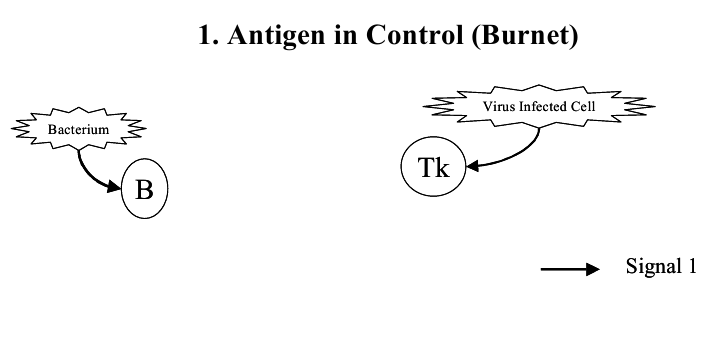
\includegraphics[width=0.75\textwidth]{img/signals1-antigen.png}
\caption{Antígeno no controle}
\end{figure}

Em algum ponto no início da vida, os linfócitos aprendiam a diferenciar o próprio, células pertencentes ao corpo, do não-próprio, células estranhas ao corpo, que deveriam ser eliminadas. As células que geravam respostas auto-imunes (reações contra as células próprias) era removidas nesse ponto, restando apenas as capazes de identificar o não-próprio.

\begin{figure}[h]
\centering
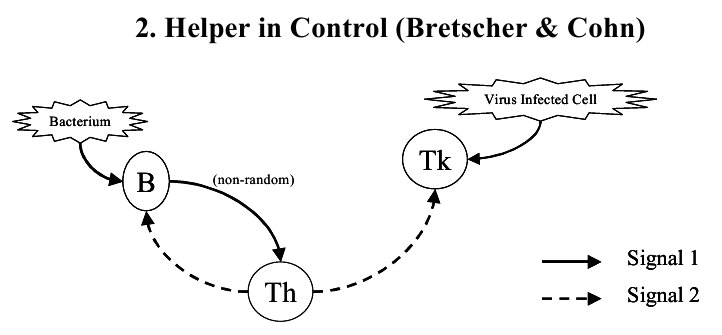
\includegraphics[width=0.75\textwidth]{img/signals2-helper.png}
\caption{Auxiliar no controle}
\end{figure}

Bretscher e Cohn introduziram uma segunda célula, o linfócito T auxiliar, ou T$_{h}$ (T \emph{helper}), que regulava a ativação dos linfócitos B. O linfócito B apresenta o antígeno ao linfócito T e aguarda sua confirmação para iniciar a resposta. A introdução dessa célula tem o objetivo de evitar uma reação auto-imune sem controle. Lafferty e Cunningham introduziram uma terceira célula, a Célula Apresentadora de Antígeno (APC, \emph{Antigen Presenting Cell}), cuja função é decompor os antígenos e apresentá-los aos linfócitos T. Dessa forma, o funcionamento das células do modelo anterior agora depende da ativação do linfócito T pela APC.

\begin{figure}[h]
\centering
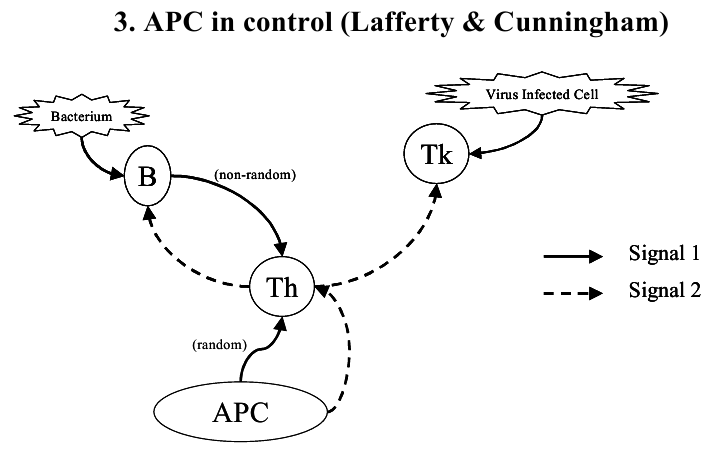
\includegraphics[width=0.75\textwidth]{img/signals3-apc.png}
\caption{APC no controle}
\end{figure}

\section{Não-próprio infeccioso}

O modelo mais aceito na imunologia atualmente, foi proposto por Janeway. Nele, as APCs também têm de ser ativadas: elas só enviam o sinal dois aos linfócitos T quando tiverem reconhecido padrões patológicos no antígeno. Assim, da mesma forma, o funcionamento do modelo anterior depende de um novo fator, antes a APC, agora o recdonhecimento de padrões pela APC.

\begin{figure}[h]
\centering
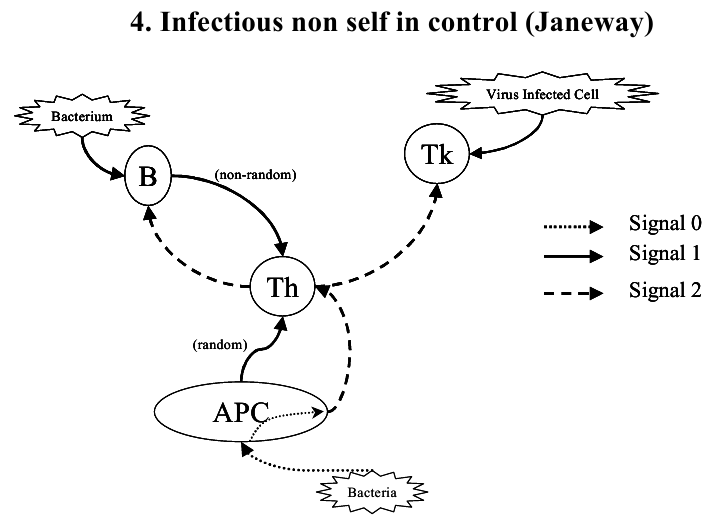
\includegraphics[width=0.75\textwidth]{img/signals4-ins.png}
\caption{Não-próprio infeccioso no controle}
\end{figure}

\section{A Teoria do Perigo}

Uma adição ainda mais recente foi a da Teoria do Perigo \cite{Matzinger1994}. Matzinger defende a teoria de que não é a separação do próprio e do não-próprio a força que impulsiona o sistema imunológico, mas sim o que ela caracteriza como ``perigo'': qualquer coisa que cause estresse ou morte não-apoptética (não natural) da célula. Embora não seja completa, essa teoria explica fenômenos que outras teorias sobre o sistema imunológico não explicavam, como o fato de não haver reação contra bactérias no intestino ou na comida, a mudança do conceito de próprio durante a vida e a problemática da própria definição do próprio e do não-próprio.

Mais do que isso, a Teoria do Perigo muda a forma como se enxerga o sistema imunológico como um todo: um sistema responsável por manter o corpo em estado de equilíbrio. Dessa forma, a distinção explícita do próprio se torna desnecessária. Discriminação ainda existe, mas seu foco é o perigo, não mais o estranho.

Uma explicação detalhada do sistema imunológico, e seu funcionamento conforme a Teoria do Perigo, é apresentado na figura 1, abaixo\footnote{MATZINGER, P. \emph{op. cit.}}. Os linfócitos B são os responsáveis pela identificação de antígenos através de receptores em sua superfície. Durante uma infecção, essas células se multiplicam e produzem anticorpos para eliminar os antígenos identificados. Elas são capazes de adaptar-se a virtualmente qualquer tipo de antígeno, gerando a resposta adequada. Um outro tipo de linfócito, os linfócitos T, quando ativados, podem exercer uma de duas funções: os linfócitos T citotóxicos (CTL) são responsáveis pela eliminação de células infectadas, enquanto que os linfócitos T auxiliares (T$_{h}$) são responsáveis pela ativação de outras células, entre elas os linfócitos B.

Além disso, alguns linfócitos T são mantidos como células de memória. Durante a resposta imunológica, os linfócitos B e T$_{h}$ se multiplicam para combater os antígenos, e são removidos quando a resposta termina. No entanto, alguns linfócitos T são mantidos, para que possam ser usados em futuras respostas ao mesmo tipo de antígeno. A combinação de linfóctios T virgens (sem um tipo de antígeno associado) e de memória permite que o sistema imunológico gere respostas tanto a novas ameaças quanto a ameaças recorrentes.

Existe ainda um outro tipo de linfócito, o T \emph{killer} (Tk), que não tem receptores antígeno-específicos, mas é capaz de reconhecer células infectadas e algumas células anormais. O objetivo dessas células é atuar como a primeira defesa contra infecções, e são muito importantes nos começo da vida.

\begin{figure}[h]
\centering
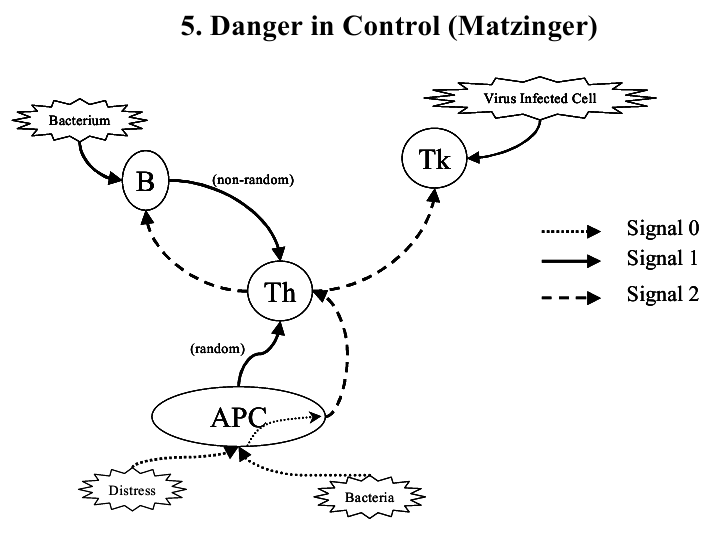
\includegraphics[width=0.75\textwidth]{img/signals5-danger.png}
\caption{Perigo no controle}
\end{figure}

O comportamento dos linfócitos T e B se baseia em três regras:

\begin{enumerate}
\item Linfócitos T e B entram em atividade ao receber os sinais um e dois, morrem ao receber apenas o sinal um e ignoram o sinal dois sem o recebimento do sinal um.
\item Linfócitos T aceitam o sinal dois apenas de APCs, enquanto os linfócitos B, apenas de linfócitos T ativos ou células de memória. O sinal um pode ter origem em qualquer célula.
\item Linfócitos T ativados não precisam do sinal dois para entrarem em ação. Após um período de tempo, elas voltam ao estado de repouso, necessitando novamente dos dois sinais.
\end{enumerate}

Células Apresentadoras de Anítgeno (ATP, ou Antigen Presenting Cell) são as células responsáveis por apresentar os antígenos às células T. Essas células podem ser os linfócitos B, macrófagos e as células dendríticas. Quando as células se encontram em estado de estresse ou morrem de forma não programada, enviam um sinal para as células APC, representado pela seta Sinal 0. Isso desencadeia o envio do sinal dois para os linfócitos Th. Enquanto isso, linfócitos B usam seus receptores para reconhecer antígenos nas suas redondezas, enviando o sinal um para os linfócitos Th. É o par de sinais um (reconhecimento do antígeno) e dois (sinal enviado pelo linfócito T, ativado pelo sinal de perigo) que faz com que a reação imunológica tenha início.

Um conceito importante da Teoria do Perigo é a tolerância. Linfócitos B que reconhecem células próprias continuamente recebem o sinal um (identificação através dos receptores em sua superfície). No entanto, essas células não apresentam perigo (não causam danos a outras células), logo o sinal dois nunca será gerado. Pela lei um acima, sem receber o sinal dois de outras células, o linfócito será removido. Dessa maneira, corpos estranhos mas que não causem dano (perigo) ao corpo não geram respostas imunes.

